\chapter{Beyond Diagnostic Classifiers: Probing Language Model Similarity} \label{chapter:svcca}

% \epigraph{``Let's travel by miles,'' advised the Humbug; ``it's shorter.''

% ``Let's travel by half inches,'' suggested Milo; ``it's quicker.''}{Norton Juster, \textit{The Phantom Tollbooth}}

\epigraph{
% ``You must be the fat man,'' said Tock, learning not to count too much on appearance.

% ``The thinnest one in the world,'' he replied brightly; ``but if you have any questions, I suggest you try the thin man, on the other side of the house.''

Just as they suspected, the other side of the house looked the same as the front, the back, and the side, and the door was again answered by a man who looked precisely like the other three.}{Norton Juster, \textit{The Phantom Tollbooth}}

In this chapter, we present the first work focused on training dynamics of modern neural language models. In order to understand how a language model learns underlying properties, such as POS and topic, over the course of training, we first experiment with diagnostic classifiers, a standard probing method. Finding these methods to be insufficiently sensitive to subtle changes in representations over the course of training, we instead introduce a method based on model similarity (Section~\ref{sec:interpretability_similarity_analysis}), comparing the representations produced by language models and models targeting the underlying properties\footnote{We like to call this method the \textbf{Similarity Probe for Intrinsic Linguistic Labels} (SPILL).}.

Using Singular Vector Canonical Correlation Analysis (SVCCA), we compare the similarity of language models (word predictors) with tag predictors at various stages of training. This analysis presents several additional advantages over contemporary probing methods. Training is far more efficient, because it consists only of matrix factorization, rather than training separate neural networks. Furthermore, we do not require parallel annotated data for evaluation, as we are interested only in the internal representations, and not in the performance, of these tag predictors.

This strategy yields a variety of informative results about the training process of the language model. We find that coarse POS is learned first, and topic information is learned last, with fine-grained POS and semantic information learned in between. Early in training, models targeting different \textit{tasks} (i.e., language modeling or tag prediction) with the same inputs tend to produce similar representations, and then specialize to their tasks. 

We also see that different layers exhibit different behavior: recurrent layer representations become more task-agnostic in late training, but embedding layers become more specialized to their task later in training. However, embedding layers nonetheless remain very generic throughout training when compared to the task-specific recurrent layers. The task-generality of embeddings may explain the effectiveness of pretrained embeddings to initialize representations for other tasks, as a task-agnostic embedding may be used transferred more easily to another environment while upper-level embeddings require more fine-tuning~\citep{howard_fine-tuned_2018}.

By investigating the language model over the full course of its training, we have a better view of how different layers specialize and the degree to which particular language properties and general input structure shapes representations.



\paragraph*{Publication Status } This work was published in NAACL 2019.


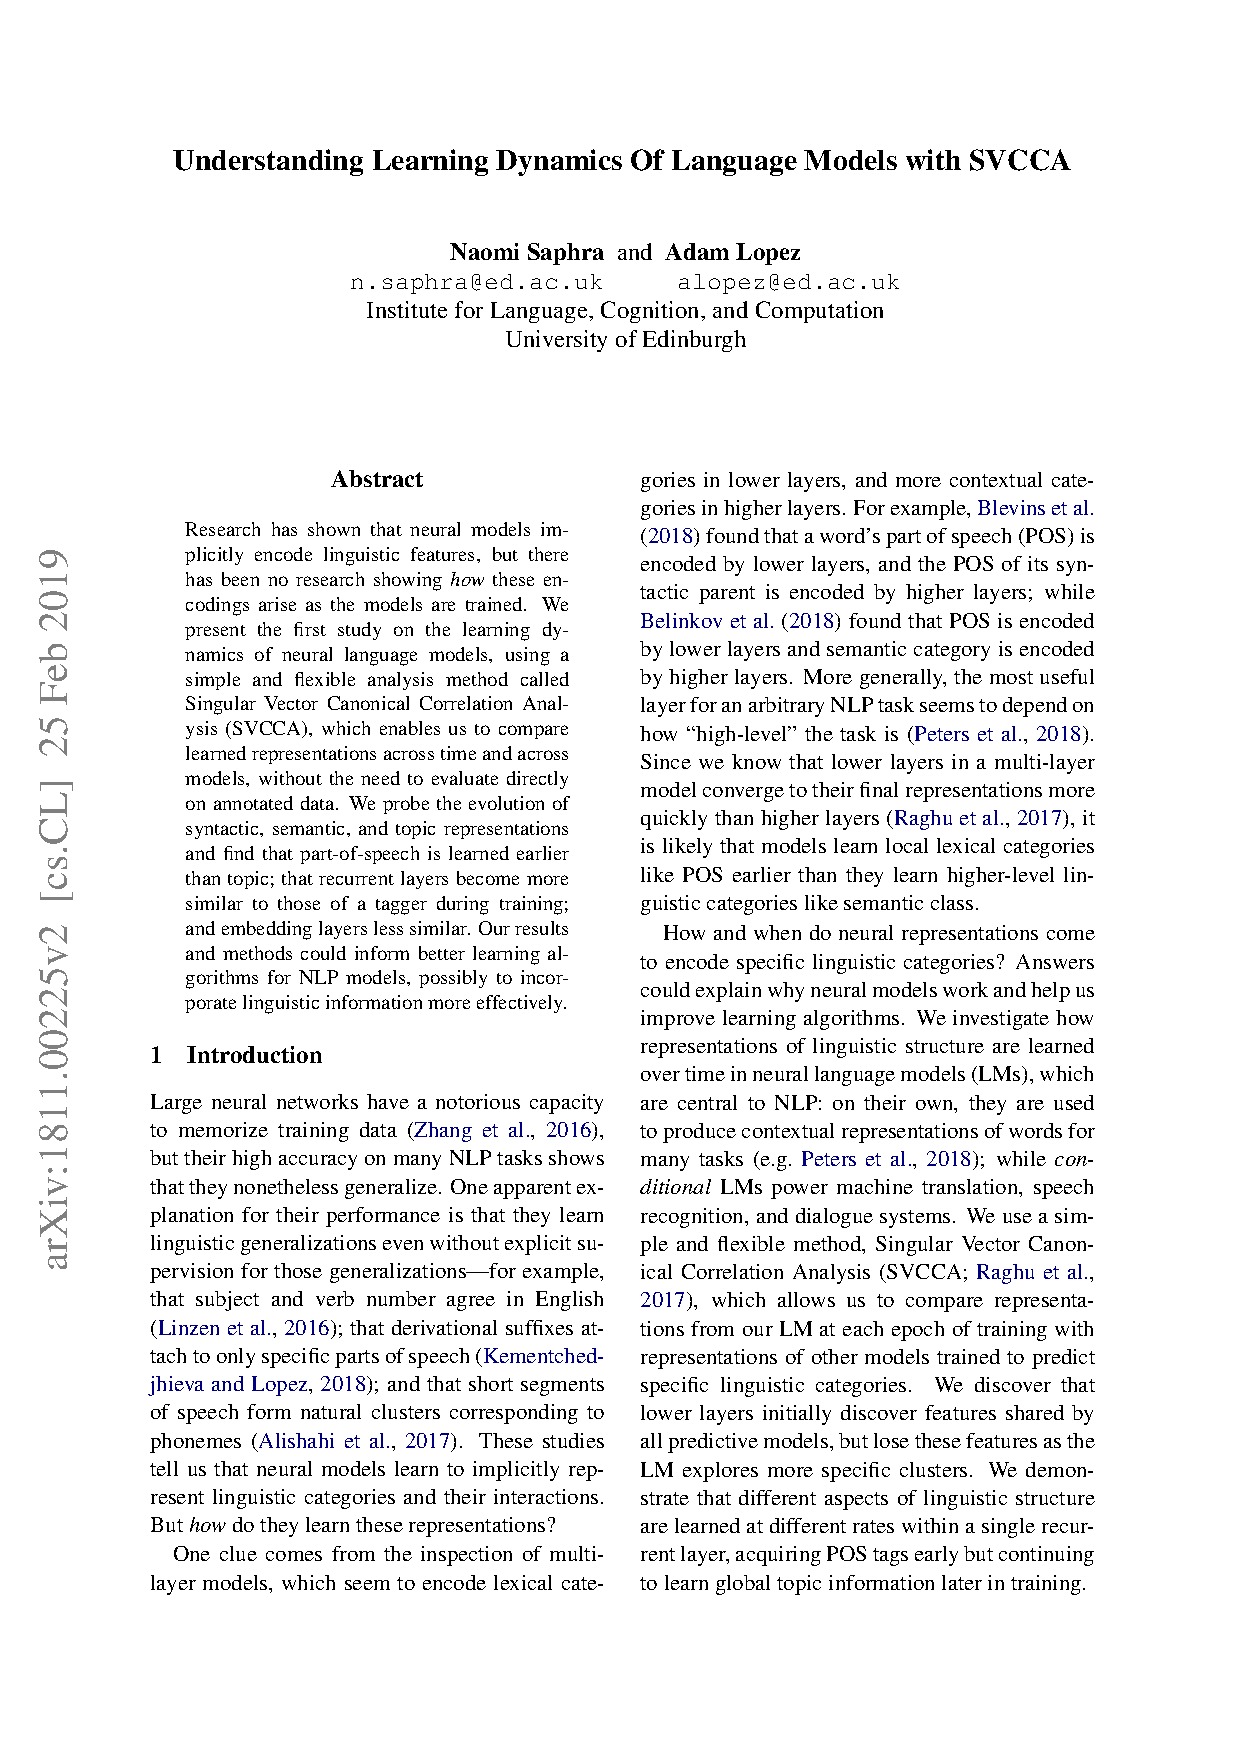
\includepdf[pages=-,pagecommand={}]{svcca/chapter.pdf}

\section{Comments on the paper}

In addition to the insights we gain from observing the time course of training, the model similarity method we use provides some intriguing insights even without considering the time dimension. When looking at input tagging instead of next-tag prediction, we find that more granular tagging produces representations that are more similar to LM representations (e.g., a model predicting simple Universal Dependencies POS tags produces more LM-like representations than a model predicting more granular PTB POS tags). This result suggests that complex tag information is retained from input words, but the structure ultimately encoded in predictions does not resemble the linguistic ontologies. We also see that input structure itself is retained, even given random target labels, based on the high baseline similarity between the language model and randomized (that is, with \textit{memorized} outputs) taggers. Results like this suggest \textit{general} properties of the LSTM, and possibly further of neural networks, in their reliance on input structure independent of output.

These insights suggest the possibility of using similarity as a general probing method, outside of training dynamics experiments--and indeed, since the publication of this paper, representational similarity methods have been widely applied in NLP. \citet{chrupala_correlating_2019} and \citet{chrupala_symbolic_2019} both explored the correlations between different vector and symbolic representations using Representational Similarity Analysis. \citet{movva_dissecting_2020} and \citet{bau_identifying_2018} used neuron-level similarity to compare models. \citet{voita_bottom-up_2019} looked at the similarity between different layers of a Transformer model using a different variant on CCA, PWCCA. \citet{singh_bert_2019}, meanwhile, compared representations in different languages using unadorned CCA, and \citet{hsu_zero_2019} used SVCCA as in our paper. \citet{chung_similarity_2020} and \citet{wu_similarity_2020} both surveyed a variety of similarity techniques, with \citet{wu_similarity_2020} validating one of the assumptions behind our method by confirming that similar architectures produced similar representations. Note that nearly all of these works postdate the work in this chapter, and almost all of them cite it.

While in general, models are more accurate when they are more similar to the same architecture trained with different seeds \citep{raghu_svcca:_2017}, it is yet to be seen whether high similarity \textit{across tasks} (e.g., LM compared to a tagging task as in this paper) indicates higher LM performance. If so, it would be interesting to see \textit{which tasks}. Can we glean information about LM performance from similarity to representations for all tasks, or only for those that involve a closer distance of dependencies (POS) or farther (topic)? This is an essential result to confirm that similarity analysis avoids one of the flaws of diagnostic classifiers: a lack of correlation between model accuracy and probe accuracy.

It is worth noting that there is no theoretical reason establishing that modules should have high similarity scores, even if they are the same type of module and situated with a similar environment in the pipeline of a model, but in practice \citep{chung_similarity_2020,raghu_svcca:_2017,morcos_insights_2018} this does seem to be the case. Therefore, although CCA yields specifically a \textit{linear} similarity, it is distinct from the common use of linear functions as probing models in that there is a clear empirical justification for the assumption that two representations  will be linearly similar, if they are accomplishing the same function (such as  representing POS as a recurrent module feeding into a softmax layer).

\subsection{Generalizing to Attentional Models}

The methods of this paper could be straightforwardly applied to any Transformer-based LM, including masked LMs rather than autoregressive. In order to do so, one would substitute the desired tag for the word being predicted and apply SVCCA to the activation vectors produced by, e.g., the feedforward layers of each Transformer module. In addition, similarity of the attention distributions used by models predicting a tag vs. a word could be measured through Shannon- or KL-divergence.